\lab{Numerical Derivatives}{Numerical Derivatives}
\label{lab:NumericalDerivatives}
\objective{Understand and implement finite difference approximations of the derivative in single and multiple dimensions. Evaluate the accuracy of these approximations.}

\section*{Derivative Approximations in One Dimension} % =======================

The derivative of a function $f$ at a point $x_0$ is

\begin{equation}
\label{eqn:deriv}
f'(x_0) = \lim_{h\rightarrow 0} \frac{f(x_0 + h)-f(x_0)}{h}.
\end{equation}
%
In this lab, we will investigate one way a computer can calculate $f'(x_0)$.

\subsection*{Forward Difference Quotient} % -----------------------------------

Suppose that in Equation \eqref{eqn:deriv}, instead of taking a limit, we just pick a small value for $h$.
Then we would expect $f'(x_0)$ to be close to the quantity
%
\begin{equation}\label{equ:forward_diff}
\frac{f(x_0 + h)-f(x_0)}{h}.
\end{equation}
%
This quotient is called the \emph{first order forward difference approximation} of the derivative.
Because $f'(x_0)$ is the limit of such quotients, we expect that when $h$ is small, this quotient is close to $f'(x_0)$.
We can use Taylor's formula to find just how close.

By Taylor's formula,
\[
f(x_0+h) = f(x_0) + f'(x_0)h + R_2(h),
\]
where $R_2(h) = \left( \int_0^1 (1-t) f''(x_0+th) dt \right) h^2$.
(This is called the \emph{integral form} of the remainder for Taylor's Theorem; see Volume 1 Chapter 6). When we solve this equation for $f'(x_0)$, we get
%
\begin{equation}\label{equ:forward_diff_with_remainder}
f'(x_0) = \frac{f(x_0+h)-f(x_0)}{h} - \frac{R_2(h)}{h}.
\end{equation}
%
Thus, the error in using the first order forward difference quotient to approximate $f'(x_0)$ is
\[
\left | \frac{R_2(h)}{h} \right | \leq |h| \int_0^1 |1 - t||f''(x_0+th)|dt.
\]
If we assume $f''$ is continuous, then for any $\delta$, set $M = \sup_{x \in (x_0-\delta, x_0+\delta)} f''(x)$. Then if $|h| < \delta$, we have
\[
\left | \frac{R_2(h)}{h} \right | \leq |h|\int_0^1 M dt = M|h|  {\in}  O(h).
\]
Therefore, the error in using \eqref{equ:forward_diff} to approximate $f'(x_0)$ grows like $h$.

\subsection*{Centered Difference Quotient} % ----------------------------------

In fact, we can approximate $f'(x_0)$ to the second order with another difference quotient, called the \emph{centered difference quotient}.  We begin by trying to find the \emph{backward difference quotient}.
Evaluate Taylor's formula at $x_0-h$ to derive
%
\begin{equation}\label{equ:backwards_diff_with_remainder}
f'(x_0) = \frac{f(x_0)-f(x_0-h)}{h} + \frac{R_2(-h)}{h}.
\end{equation}
%
The first term on the right hand side of \eqref{equ:backwards_diff_with_remainder} is called the \emph{backward difference quotient.}
This quotient also approximates $f'(x_0)$ to first order, so it is not the quotient we are looking for.
When we add \eqref{equ:forward_diff_with_remainder} and \eqref{equ:backwards_diff_with_remainder} and solve for $f'(x_0)$ (by dividing by 2), we get
%
\begin{equation}\label{equ:centered_diff}
f'(x_0) = \frac{\frac{1}{2}f(x_0+h) - \frac{1}{2}f(x_0-h)}{h} + \frac{R_2(-h) - R_2(h)}{2h}
\end{equation}
%
The \emph{centered difference quotient} is the first term of the right hand side of \eqref{equ:centered_diff}.
Let us investigate the remainder term to see how accurate this approximation is.
Recall from the proof of Taylor's theorem that $R_k = \frac{f^{(k)}(x_0)}{k!}h^k + R_{k+1}$. Therefore,
%
\begin{align*}
\frac{R_2(-h) - R_2(h)}{2h} &= \frac{1}{2h}\left(\frac{f''(x_0)}{2}h^2 + R_{3}(-h) - \frac{f''(x_0)}{2}h^2 - R_{3}(h) \right)\\
&= \frac{1}{2h} ( R_3(-h)-R_3(h))\\
&= \frac{1}{2h}\left(  \left( \int_0^1 \frac{(1-t)^2}{2} f'''(x_0+th) dt \right) h^3  -  \left(\int_0^1 \frac{(1-t)^2}{2} f'''(x_0-th) dt \right) h^3  \right)\\
&= \left(  \int_0^1 \frac{(1-t)^2}{4}( f'''(x_0+th)-f'''(x_0-th)) \right)h^2\\
&{\in}   O(h^2)
\end{align*}
%
once we restrict $h$ to some $\delta$-neighborhood of 0.
So the error in using the centered difference quotient to approximate $f'(x_0)$ grows like $h^2$, which is smaller than $h$ when $|h|<1$.

\subsection*{Accuracy of Approximations} % ------------------------------------

Let us discuss what step size $h$ we should plug into the difference quotients to get the best approximation to $f'(x_0)$.
Since $f'$ is defined as a limit as $h \rightarrow 0$, you may think that it is best to choose $h$ as small as possible, but this is not the case.
In fact, dividing by very small numbers causes errors in floating point arithmetic.
This means that as we decrease $|h|$, the error between $f'(x_0)$ and the difference quotient will first decrease, but then increase when $|h|$ gets too small because of floating point arithmetic.

Here is an example with the function $f(x) = e^x$. A quick way to write $f$ as a function in Python is with the \li{lambda} keyword.

\begin{lstlisting}
>>> import numpy as np
>>> from matplotlib import pyplot as plt
>>> f = lambda x: np.exp(x)
\end{lstlisting}

In general, the line \li{f = lambda <params> : <expression>} is equivalent to defining a function \li{f} that accepts the parameters \li{params} and returns \li{expression}.

Next we fix a step size \li{h} and define an approximation to the derivative of \li{f} using the \emph{centered difference quotient}.

\begin{lstlisting}
>>> h = 1e-1
>>> Df_app = lambda x: .5*(f(x+h)-f(x-h))/h
\end{lstlisting}

Finally, we check the accuracy of this approximation at $x_0=1$ by computing the difference between \li{Df_app(1)} and the actual derivative evaluated at 1.

\begin{lstlisting}
# Since f(x) = e^x, the derivative of f(x) is f(x)
>>> np.abs( f(1)-Df_app(1) )
0.0045327354883726301
\end{lstlisting}

We note that our functions \li{f} and \li{Df_app} behave as expected when they are passed a NumPy array.

\begin{lstlisting}
>>> h = np.array([1e-1, 1e-3, 1e-5, 1e-7, 1e-9, 1e-11])
>>> np.abs( f(1)-Df_app(1) )
array([  4.53273549e-03,   4.53046679e-07,   5.85869131e-11,
         5.85873572e-11,   6.60275079e-09,   1.04294937e-05])
\end{lstlisting}

These results are summarized in Table \ref{table:approx_errors}.

\begin{table}
\begin{center}
\begin{tabular}{|c|c|c|c|c|c|c|}
    \hline
    $h$     & 1e-1 & 1e-3 & 1e-5  & 1e-7  & 1e-9 & 1e-11 \\ \hline
    Error   & 5e-3 & 5e-7 & 6e-11 & 6e-11 & 7e-9 & 1e-5  \\ \hline
\end{tabular}
\caption{This table shows that it is best not to choose $h$ too small when you approximate derivatives with difference quotients.
Here, ``Error'' equals the absolute value of $f'(1)-f_{app}(1)$ where $f(x) = e^x$ and $f_{app}$ is the centered difference approximation to $f'$.}
\label{table:approx_errors}
\end{center}
\end{table}

Thus, the optimal value of $h$ is one that is small, but not too small. A good choice is \li{h = 1e-5}.

\begin{problem}
Write a function that accepts as input a callable function object \li{f}, an array of points \li{pts}, and
a keyword argument \li{h} that defaults to \li{1e-5}.
Return an array of the \emph{centered difference quotients} of \li{f} at each point in \li{pts} with the specified value of \li{h}.
\end{problem}

\begin{problem}
Write a function that accepts as input a callable function object \li{f}, the derivative \li{df} of the function \li{f}, an array of points \li{pts}, and
a keyword argument \li{h} that defaults to \li{1e-5}.  Return an array of the errors for the \emph{centered difference quotients} at each point in \li{pts} with the specified value of \li{h}.
\end{problem}

\begin{problem}
Use the \emph{centered difference quotient} to approximate the derivative of $f(x) = (\sin(x)+1)^x$ at $x = \frac{\pi}{3}, \frac{\pi}{4},$ and $\frac{\pi}{6}$.  Calculate the error of the approximations.
\end{problem}

You may wonder if the forward or backward difference quotients are ever used, since the centered difference quotient is a more accurate approximation of the derivative.
In fact, there are some functions that in practice do not behave well under centered difference quotients.
In these cases, one must use the forward or backward difference quotient.

Finally, we remark that forward, backward, and centered difference quotients can be used to approximate higher-order derivatives of $f$.
However, taking derivatives is an \emph{unstable} operation.
This means that taking a derivative can amplify the arithmetic error in your computation.
For this reason, difference quotients are not generally used  to approximate derivatives higher than second order.

\begin{problem}
The radar stations A and B, separated by the distance a = 500 m, track the plane C by recording the angles $\alpha$ and $\beta$ at one-second intervals (See figure \ref{plane} ).
Three successive readings are give in table \ref{angles}.
Use central difference quotients to calculate the speed v of the plane and the climb angle $\gamma$ at t = 10 s.
The coordinates of the plane can be shown to be
\begin{equation}
x = a \frac{\tan(\beta)}{\tan(\beta)-\tan(\alpha)}
\end{equation}

\begin{equation}
 y = a \frac{\tan(\beta)\tan(\alpha)}{\tan(\beta)-\tan(\alpha)}
\end{equation}


(Kiusalaas, Jaan. Numerical Methods in Engineering with Python 3)
\end{problem}

\begin{figure}
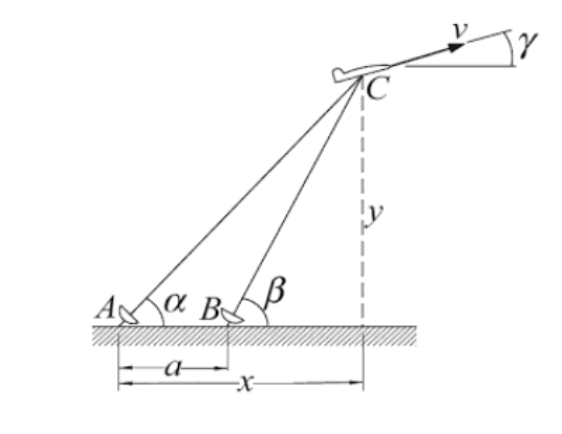
\includegraphics[width=.5\textwidth]{plane_diagram.png}
\caption{Radar stations in relation to plane}
\label{plane}
\end{figure}

\begin{figure}
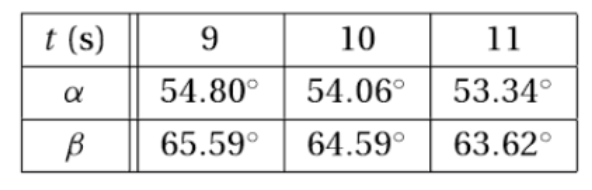
\includegraphics[width=.5\textwidth]{angles_table.png}
\caption{Angles $\alpha$ and $\beta$ at one-second intervals}
\label{angles}
\end{figure}

\section*{Derivative Approximations in Multiple Dimensions} % =================

Finite difference methods can also be used to calculate derivatives in higher dimensions.
Recall that the Jacobian of a function $f:\mathbb{R}^n \rightarrow \mathbb{R}^m$ at a point $x_0 \in \mathbb{R}^n$ is the $m \times n$ matrix $J = (J_{ij})$ defined component-wise by
\begin{equation*}
J_{ij} = \frac{\partial f_i}{\partial x_j}(x_0).
\end{equation*}
For example, the Jacobian for a function $f:\mathbb{R}^3 \rightarrow \mathbb{R}^2$ is defined by

\[
J = \begin{pmatrix}
\frac{\partial f}{\partial x_1}&\frac{\partial f}{\partial x_2}&\frac{\partial f}{\partial x_3}
\end{pmatrix}
= \begin{pmatrix}
\frac{\partial f_1}{\partial x_1}&\frac{\partial f_1}{\partial x_2}&\frac{\partial f_1}{\partial x_3}\\
\frac{\partial f_2}{\partial x_1}&\frac{\partial f_2}{\partial x_2}&\frac{\partial f_2}{\partial x_3}
\end{pmatrix}.
\]

The Jacobian is useful in many applications.  For example, the Jacobian can be used to find zeros of functions in multiple variables.

The forward difference quotient for approximating a partial derivative is
\begin{equation*}
\frac{\partial f}{\partial x_j} (x_0) \approx \frac{f(x_0+h e_j)-f(x_0)}{h},
\end{equation*}
where $e_j$ is the $j^{th}$ standard basis vector.
Similarly, the centered difference approximation is
\begin{equation*}
\frac{\partial f}{\partial x_j} (x_0) \approx \frac{\frac{1}{2}f(x_0+h e_j)-\frac{1}{2}f(x_0-h e_j)}{h}.
\end{equation*}

\begin{problem}
\leavevmode
Write a function that accepts
\begin{enumerate}
\item a function handle \li{f},
\item an integer \li{n} that is the dimension of the domain of \li{f},
\item an integer \li{m} that is the dimension of the range of \li{f},
\item an \li{1 x n}-dimensional NumPy array \li{pt} representing a point in $\mathbb{R}^n$, and
\item a keyword argument \li{h} that defaults to \li{1e-5}.
\end{enumerate}
Return the approximate Jacobian matrix of \li{f} at \li{pt} using the centered difference quotient.
\end{problem}
\begin{problem}
\item Let $f: \mathbb{R}^2 \to \mathbb{R}^2$ be defined by
%
\begin{equation*}
f(x, y) =
\left[\begin{array}{c}
e^{x} \sin(y) + y^3 \\
3y - \cos(x)
\end{array}\right]
\end{equation*}
%
Find the error between your Jacobian function and the analytically computed derivative on the square $[-1,1] \times [-1,1]$ using ten thousand grid points (100 per side).
You may apply your Jacobian function to the points one at a time using a double \li{for} loop.  Once you get the error matrix for a given point, calculate the Frobenius norm of this matrix (\li{la.norm} defaults to the Frobenius norm).  This norm will be your total error for that point.
What is the maximum error of your Jacobian function over all points in the square?

Hint: The following code defines the function
$f(x,y) = \left[\begin{array}{c} x^2 \\ x+y \end{array}\right]$.

\begin{lstlisting}
# f accepts a length-2 NumPy array
>>> f = lambda x: np.array([x[0]**2, x[0]+x[1]])
\end{lstlisting}
\end{problem}

% =============================================================================
% OLD IMAGE FILTER MATERIAL (might work well in Fourier 2 lab?) ===============
% =============================================================================

\begin{comment}
\section*{Image Filters} % ====================================================

Recall that a computer stores an image as a 2-D array of pixel values (i.e., a matrix of intensities).
An image filter is a function that transforms an image by operating on it locally.
That is, to compute the $ij^{th}$ pixel value in the new image, an image filter uses only the pixels in a small neighborhood around the $ij^{th}$ pixel in the original image.

In this lab, we will use a filter derived from the gradient of an image to find edges in an image.

\subsection*{Convolutions} % --------------------------------------------------

One example of an image filter is to \emph{convolve} an image with a filter matrix.
A filter matrix is a matrix whose height and width are relatively small odd numbers.
If the filter matrix is
\[
F = \begin{pmatrix}
f_{-1,-1}&f_{-1,0}&f_{-1,1}\\
f_{0,-1}&f_{0,0}&f_{0,1}\\
f_{1,-1}&f_{1,0}&f_{1,1}
\end{pmatrix},
\]
then the convolution of an image $A$ with $F$ is $A \ast F = (C_{ij})$ where
\begin{equation}\label{equ:convolve}
C_{ij} = \sum_{k=-1}^1 \sum_{\ell=-1}^1 f_{k\ell}A_{i+k,j+\ell}.
\end{equation}
Say $A$ is an $m \times n$ matrix. Here, we take $A_{ij}=0$ when $i \not \in \{1, \ldots m\}$ or $j \not \in \{1, \ldots, n\}$.
The value of $C_{ij}$ is a linear combination of the nearby pixel values, with coefficients given by $F$ (see Figure \ref{fig:convolution}).
In fact, $C_{ij}$ equals the Frobenius inner product of $F$ with the $3 \times 3$ submatrix of $A$ centered at $ij$.

\begin{figure}
\centering
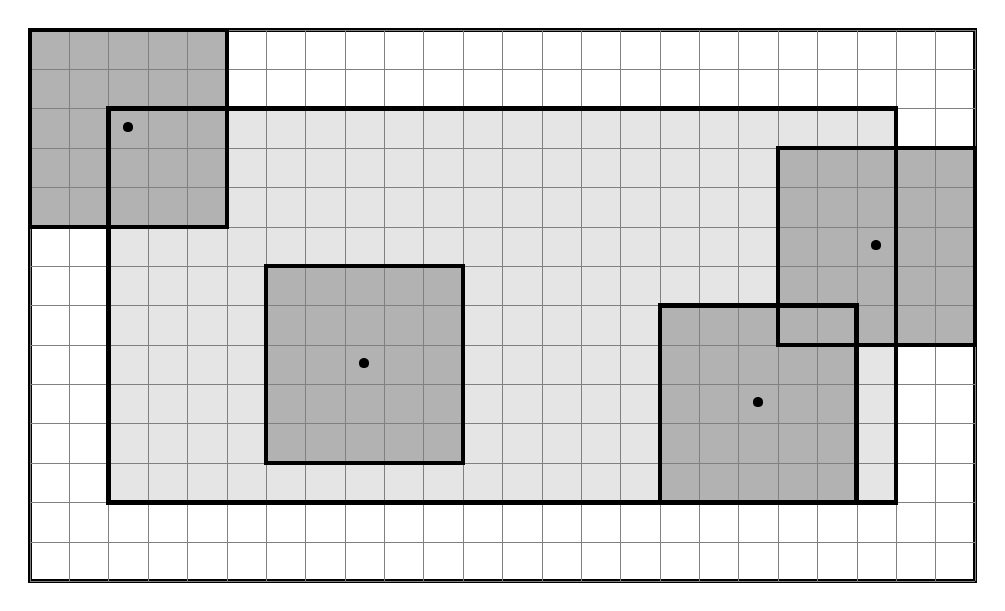
\begin{tikzpicture}
\node[draw, minimum width=12cm, minimum height=
    7cm, ultra thick](outer_rec)[]{};
\node[draw, minimum width=10cm, minimum height=
    5cm, ultra thick, fill=black!10!](inner_rec)[]{};
\node[draw, minimum width=2.5cm, minimum height=2.5cm,
    ultra thick, fill=black!30!](square1)at(-4.75,2.25){\textbullet};
\node[draw, minimum width=2.5cm, minimum height=2.5cm,
    ultra thick,fill=black!30!](square2)at(-1.75,-.75){\textbullet};
\node[draw, minimum width=2.5cm, minimum height=2.5cm,
    ultra thick, fill=black!30!](square3)at(4.75,.75){\textbullet};
\node[draw, minimum width=2.5cm, minimum height=2.5cm,
    ultra thick, fill=black!30!](square4)at(3.25,-1.25){\textbullet};
\draw[step=.5, ultra thin, color=black!50!](-6,-3.5)grid(6,3.5);

%redraw borders
\node[draw, minimum width=10cm, minimum height=
    5cm, ultra thick, ][]{};
\node[draw, minimum width=2.5cm, minimum height=2.5cm,
    ultra thick]at(-4.75,2.25){};
\node[draw, minimum width=2.5cm, minimum height=2.5cm,
    ultra thick]at(-1.75,-.75){};
\node[draw, minimum width=2.5cm, minimum height=2.5cm,
    ultra thick]at(4.75,.75){};
\node[draw, minimum width=2.5cm, minimum height=2.5cm,
    ultra thick]at(3.25,-1.25){};
\end{tikzpicture}
\caption{This diagram illustrates how to convolve an image with a filter.
The light grey rectangle represents the original image $A$, and the dark grey squares are the filter $F$.
The larger rectangle is the image padded with zeros; i.e., all pixel values in the outer white band are 0.
To compute the entry of the convolution matrix $C$ located at a black dot, take the inner product of $F$ with the submatrix of the padded image centered at the dot.}
\label{fig:convolution}
\end{figure}

\subsubsection*{Implementation in NumPy} % - - - - - - - - - - - - - - - - - -

Let us write a function that convolves an image with a filter.
You can test this function on the image \li{cameraman.jpg}, which appears in Figure \ref{fig:cameraman}.
The following code loads this image and plots it with matplotlib.

\begin{lstlisting}
>>> image = plt.imread('cameraman.jpg')
>>> plt.imshow(image, cmap = 'gray')
>>> plt.show()
\end{lstlisting}

Here is the function definition and some setup.

\begin{lstlisting}
1. def Filter(image, F):
2.     m, n = image.shape
3.     h, k = F.shape
\end{lstlisting}

To convolve \li{image} with the filter \li{F}, we must first \emph{pad} the array \li{image} with zeros around the edges.
This is because in \eqref{equ:convolve}, entries $A_{ij}$ are set to zero when $i$ or $j$ is out of bounds.
We do this by creating a larger array of zeros, and then making the interior part of the array equal to the original image (see Figure \ref{fig:convolution}).

For example, if the filter is a $3 \times 3$ matrix, then the following code will pad the matrix with the appropriate number of zeros.

\begin{lstlisting}
 # Create a larger matrix of zeros
image_pad = np.zeros((m+2, n+2))
# Make the interior of image_pad equal to the original image
image_pad[1:1+m, 1:1+n] = image
\end{lstlisting}

We want to do this in general in our function.  Note that the number of zeros we need to pad our array depends on the size of the filter \li{F}.

\begin{lstlisting}
5.    image_pad = # Create an array of zeros of the appropriate size
6.   # Make the interior of image_pad equal to image
\end{lstlisting}

Finally, we iterate through the image to compute each entry of the convolution matrix.

\begin{lstlisting}
7.    C = np.zeros(image.shape)
8.    for i in range(m):
9.        for j in range(n):
10.            C[i,j] = # Compute C[i, j]
\end{lstlisting}

\subsubsection*{Gaussian Blur} % - - - - - - - - - - - - - - - - - - - - - - -

A \emph{Gaussian blur} is an image filter that operates on an image by convolving with the matrix
\[
G = \frac{1}{159}\begin{pmatrix}
2&4&5&4&2\\
4&9&12&9&4\\
5&12&15&12&5\\
4&9&12&9&4\\
2&4&5&4&2
\end{pmatrix}.
\]

Blurring an image can remove ``noise'', or random variation that is the visual analog of static in a radio signal (and equally undesirable).

\begin{problem}\label{prob:filter}
\leavevmode
Finish writing the function \li{Filter} by filling in lines 5, 6, and 10.  Hint: Note in \ref{equ:convolve}, $C_{ij}$ was calculated by summing from -1 to 1.  This is only the case if the filter \li{F} is $3 \times 3$. A slight modification is needed in the general case.  Test your function on the image \li{cameraman.jpg} using the Gaussian Blur. The result is in Figure \ref{fig:cameraman_blur}.
\end{problem}

% TODO: make pictures that aren't pdfs
\begin{figure}
\centering
\begin{subfigure}[b]{.49\textwidth}
\centering
\includegraphics[width=\textwidth]{figures/cameraman.jpg}
\caption{Unfiltered image.}
\label{fig:cameraman}
\end{subfigure}
\begin{subfigure}[b]{.49\textwidth}
\centering
\includegraphics[width=\textwidth]{figures/cameramanBlur.pdf}
\caption{Image after Gaussian blur is applied.}
\label{fig:cameraman_blur}
\end{subfigure}
\begin{subfigure}[b]{.49\textwidth}
\centering
\includegraphics[width=\textwidth]{figures/edges.pdf}
\caption{Image after the Sobel filter is applied.}
\label{fig:cameraman_edges}
\end{subfigure}
\caption{Here is an example of a Gaussian blur and the Sobel filter applied to an image.
This photo, known as ``cameraman,'' is a standard test image in image processing.
A database of such images can be downloaded from \url{http://www.imageprocessingplace.com/root_files_V3/image_databases.htm}.}
\label{fig:cameraman1}
\end{figure}

\subsection*{Edge Detection} % ------------------------------------------------

Automatic detection of edges in an image can be used to segment or sharpen the image.
We will find edges with the Sobel filter, which computes the gradient of the image at each pixel.
The magnitude of the gradient tells us the rate of change of the pixel values, and so large magnitudes should
correspond to edges within the image.
The Sobel filter is not a convolution, although it does use convolutions.

We can think of an image as a function from a $2 \times 2$ grid of points to $\mathbb{R}$.
The image maps a pixel location to an intensity.
It does not make sense to define the derivative of this function as a limit because the domain is discrete---a step size $h$ cannot take on arbitrarily small values.
Instead, we \emph{define} the derivative to be the centered difference quotient of the previous section.
That is, we define the derivative in the $x$-direction at the $ij^{th}$ pixel to be
\[
\frac{1}{2}A_{i+1, j} - \frac{1}{2}A_{i-1, j}.
\]

We can use a convolution to create a matrix $A_x$ whose $ij^{th}$ entry is the derivative of $A$ at the $ij^{th}$ entry, in the $x$-direction.
In fact, $A_x = A \ast S$, where
\[
S = \frac{1}{8}
\left[\begin{array}{ccc}
-1 & 0 & 1\\
-2 & 0 & 2\\
-1 & 0 & 1
\end{array}\right].
\]

Note that this convolution takes a weighted average of the $x$-derivatives at $(i, j)$, $(i, j+1)$, and $(i, j-1)$.
The derivative at $(i, j)$ is weighted by 2.
Using a weighted average instead of just the derivative at $(i, j)$ makes the derivative less affected by noise.

Now we can define the Sobel filter.
A Sobel filter applied to an image $A$ results in an array $B = (B_{ij})$ of 0's and 1's, where the 1's trace out the edges in the image.
By definition,
\[
B_{ij} = \left\{
     \begin{array}{ll}
       1 & \text{if}\; \;\|\nabla A(ij)\|_2 > M \\
       0 & \text{otherwise}.
     \end{array}
   \right.
\]
Here, $\nabla A(ij) = ((A \ast S)_{ij}, (A\ast S^T)_{ij})$ is the gradient of $A$ at the $ij^{th}$ pixel.
The constant $M$ should be ``sufficiently large'' enough to pick out those pixels with the largest gradient (i.e., those pixels that are part of an edge).
A good choice for $M$ is 4 times the average value of $\|\nabla A(ij)\|_2$ over the whole image $A$.

When the Sobel filter is applied to \li{cameraman.jpg}, we get the image in Figure \ref{fig:cameraman_edges}.
Here, the 1's in $B$ were mapped to ``white'' and the 0's were mapped to ``black.''

\begin{problem}
Write a function that accepts an image as input and applies the Sobel filter to the image.  Test your function on \li{cameraman.jpg}.  Hint: If you want to find the average of a matrix \li{A}, use the function \li{A.mean()}.
\end{problem}
\end{comment}


